\documentclass[a4paper]{article}
\usepackage{lipsum}
\usepackage{url}
\usepackage{graphicx}
\usepackage{indentfirst}
\usepackage{xcolor}
\usepackage[margin=2cm]{geometry}
\graphicspath{ {images/} }

%Custom Commands
\newcommand{\Pokemon}{Pok\'{e}mon}

%NOTE: 2,000 Words / 4 Pages
%TODO: Also need to do ethics checklist
%TODO: Get a better font and layout :P
%TODO: Think of a title
%NOTE: Make the Work Plan codes more detailed
%TODO: Rewrite the Work Plan Descriptions
%TODO: Remove no cite command and check for proper references

\begin{document}

%Title Information
\title{
    Project Proposal
    \\ \large{G54IRP/COMP4027}
    \\ \large{Project Title: NEED TO THINK OF A TITLE}\vspace{-3ex}}
\author{4262648 Benjamin Charlton (psybc3)}
\date{\vspace{-2ex}12\textsuperscript{th} October 2017}
\maketitle

\section{Background and Motivation}
The following text is filler for now.
\par
\lipsum[1-7]

\section{Aims and Objectives}
The following text is filler for now.
\par
\lipsum[1-5]
\bigbreak
The objectives of this project are:
\begin{enumerate}
    \item \lipsum[1]
    \item \lipsum[1]
\end{enumerate}

\section{Work Plan}
To help outline the project flow and I have created a gantt chart (found in the appendix) and the following descriptions of each portion.

%Explanations of all of the Points on the work plan
\begin{description}
\item [\large{Documentation}]
\item [D1 - Project Proposal Draft]
Write the project proposal draft for approval and feedback from supervisor, due 12\textsuperscript{th} October.
\item [D2 - Project Proposal]
Any revisions to the project proposal that need to be made after supervisor feedback, due 22\textsuperscript{rd} October.
\item [D3 - Preliminary Ethics Checklist]
Fill out and submit the preliminary ethics checklist, no further ethical checks should be required so no further time is scheduled.

\item [Interim Report]
\colorbox{yellow}{Write the interim report summarising the work so far, due 7\textsuperscript{th} December.}
\item [Structure Sections]
\colorbox{yellow}{Decide and begin to structure the sections and the arguments within them for the final dissertation.}
\item [Research Paper]
\colorbox{yellow}{Write the final research paper, due 12\textsuperscript{th} April.}

\item [\large{Research}]
\item [R1 - Research for Proposal]
\colorbox{green}{WRITE THIS}

\item [\large{Development}]
\item [S1 - NEED TO THINK OF THESE]
\colorbox{green}{WRITE THIS}

\item [\large{Presentation}]
\item [P1 - Work on Presentation]
\colorbox{green}{WRITE THIS}
\item [P3 - Create Demo for Presentation]
\colorbox{green}{WRITE THIS}
\item [P3 - Finalise Presentation]
\colorbox{green}{WRITE THIS}
\item [P4 - Present Presentation]
\colorbox{green}{WRITE THIS}

\item [\large{Miscellaneous}]
\item [M1 - Create Git repository]
\colorbox{green}{WRITE THIS}
\item [M3 - Set up LaTeX files]
\colorbox{green}{WRITE THIS}
\item [M3 - SET/SEM Questionaries]
\colorbox{green}{WRITE THIS}

\item [\large{Other Commitments}]
\item [C1 - Welcome Weeks]
First weeks of the academic year, time set aside to allow for settling in as well as running various welcome events.
\item [C2 - Christmas Holiday]
Time off after Autumn term, Partially set aside to all for a break and time to relax..
\item [C3 - Autumn Exams]
Potentially could have exams during the entire 2 weeks so is set aside to allow for revision and the exams themselves.
This can be updated to give a better reflection of when exams will be at a later date.
\item [C4 - Easter Holiday]
Time off after Spring term, As no teaching is happening will give more time to concentrate on coursework and the presentation.
\end{description}

\section{Appendix}
%Bibliography
\nocite{*}
\bibliography{ProjectProposal}
\bibliographystyle{plain}

%Work Plan
\clearpage
\begin{center}
    \Large{Work Plan}\\
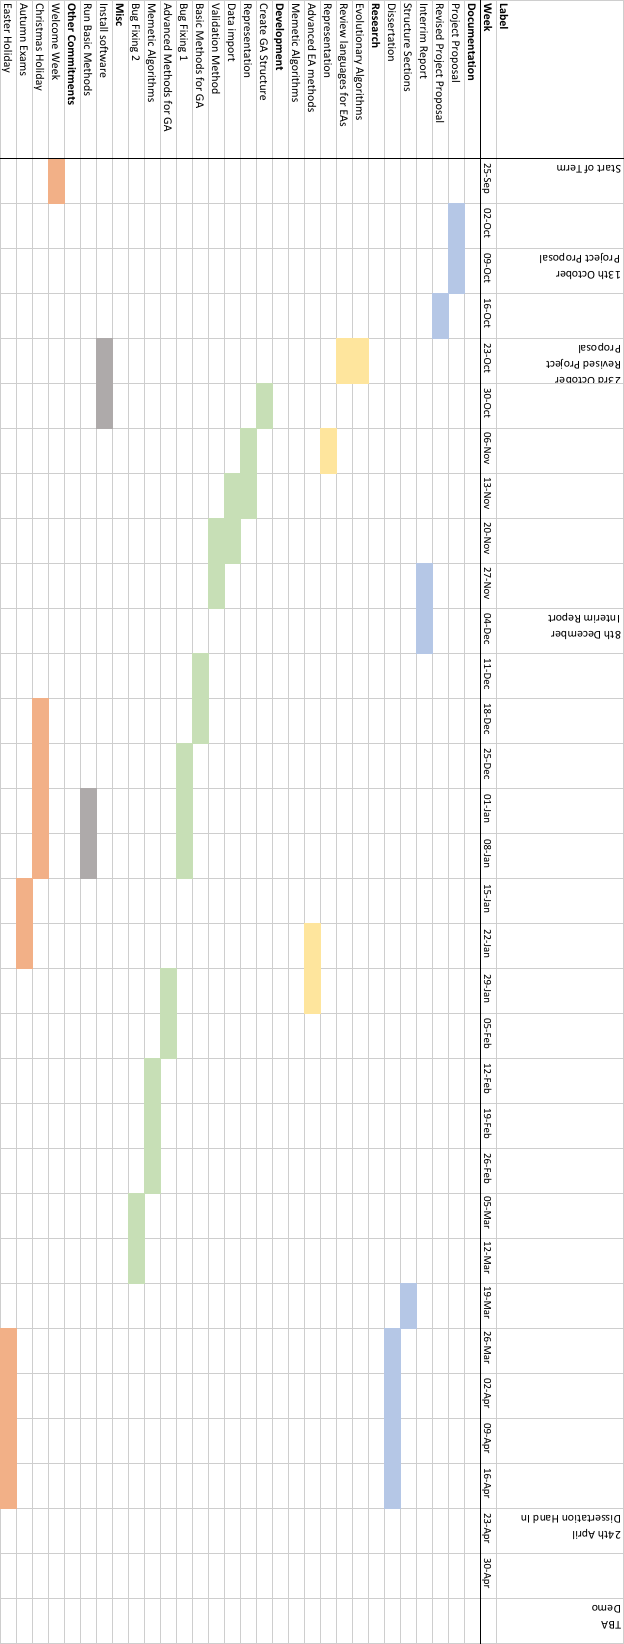
\includegraphics[height=24.8cm]{workPlanOLD.png}
\end{center}


\end{document}
